\documentclass{beamer}
\setbeamertemplate{section in toc}[sections numbered]

\usepackage[utf8]{inputenc}
\usepackage[croatian]{babel}
\usepackage[T1]{fontenc}
\usepackage{lmodern}

\usepackage{mathtools}
\usepackage{listings}
\usepackage{tikz-uml}
\usepackage{multirow}
\usepackage{tikz}
\usepackage{svg}

\usetheme[numbering=fraction]{metropolis}

\title{Sybil napadi u društvenim mrežama i zaštita od njih}
\author{Antun Razum\\Voditelj: prof. dr. sc. Siniša Srbljić}
\institute{Fakultet elektrotehnike i računarstva}
\date{\today}

\begin{document}

\maketitle

\begin{frame}{Sadržaj}
  \tableofcontents
\end{frame}

\section{Uvod}

\begin{frame}{Sybil napadi}
  \begin{itemize}
    \item \textit{Sybil} -- prema istoimenoj knjizi o ženi s disocijativnim poremećajem osobnosti
    \item napadi na distribuiranim sustavima poput senzorskih i \textit{peer-to-peer} mreža
    \item napadač stvara velik broj lažnih identiteta preko kojih utječe na ponašanje sustava
    \item danas veoma aktualno na društvenim mrežama
  \end{itemize}
\end{frame}

\begin{frame}{Primjeri}
  \begin{itemize}
    \item širenje spam sadržaja na društvenim mrežama -- često maliciozni sadržaj
    \item korištenje velikog broja lažnih identiteta za postizanje nekih "ciljeva", npr. glasanje, podizanje reputacije, lažno prijavljivanje sadržaja
    \item prosječno 20\% zahtjeva za prijateljstvo od lažnih profila bude prihvaćeno
  \end{itemize}
\end{frame}

\section{Povijest i motivacija}

\begin{frame}{Središnji autoritet}
  \begin{itemize}
    \item izdaje i provjerava podatke jedinstvene stvarnom čovjeku
    \item zahtijevanje osobnih podataka (npr. broj osobne iskaznice) ili plaćanje registracije
    \item nepoželjno jer odbija velik broj korisnika
    \item problem oko odabira središnjeg autoriteta
    \item može biti \textit{signle point of failure}
  \end{itemize}
\end{frame}

\begin{frame}{Decentralizirani pristupi}
  \begin{itemize}
    \item povezivanje korisnika s IP adresom -- lagano se može ukrasti i iskoristiti veći broj različitih IP adresa
    \item zagonetke koje zahtijevaju ljudski napor (npr. \textit{CAPTCHA}) -- predstavljanje na vlastitoj stranici ili plaćanje jeftinih servisa za rješavanje
  \end{itemize}
\end{frame}

\begin{frame}{Motivacija}
  \begin{itemize}
    \item predložene metode su ograničene
    \item omogućuju smanjenje, ali ne i eliminaciju sybil napada
    \item potrebna obrana temeljena na analizi grafa društvene mreže
  \end{itemize}
\end{frame}

\section{Pojmovi i definicije}

\begin{frame}{Model društvene mreže}
  \begin{itemize}
    \item neusmjereni beztežinski graf -- čvorovi su korisnici, a bridovi odnosi među njima, npr. prijateljstva
    \item \textit{pošteni čvorovi} -- predstavljaju stvarne korisnike mreže
    \item \textit{sybil čvorovi} -- lažni identiteti stvoreni od strane napadača
    \item \textit{napadački bridovi} -- bridovi između sybil čvorova i poštenih čvorova
    \item \textit{sybil regija} sastoji se od svih sybil čvorova, a \textit{poštena regija} od svih poštenih čvorova
  \end{itemize}
\end{frame}

\begin{frame}{Model društvene mreže}
  \begin{figure}[h]
    \centering
    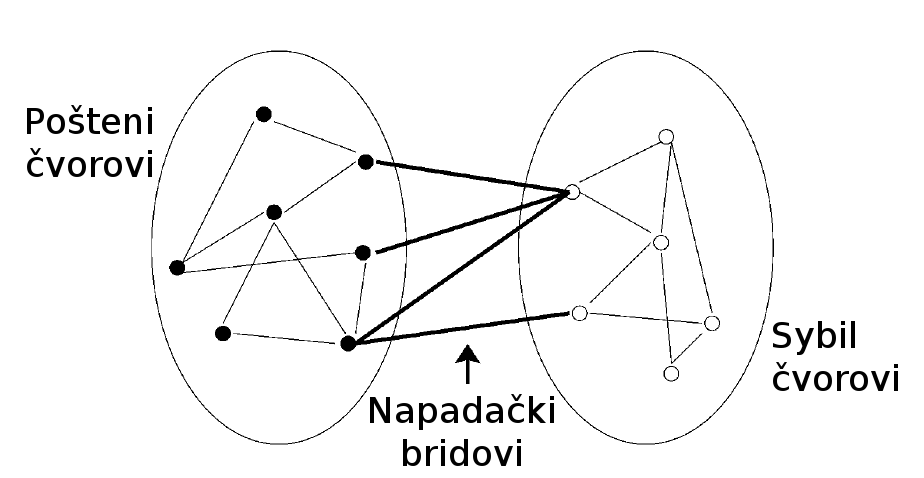
\includegraphics[scale=0.3]{attack.png}
  \end{figure}
\end{frame}

\begin{frame}{Slučajne šetnje}
  \begin{itemize}
    \item \textit{slučajna šetnja} -- šetnja u grafu s nasumično odabranim prijelazima
    \item slučajne šetnje su \textit{ergodične} -- konvergiraju prema \textit{stacionarnoj distribuciji} kada im duljina teži u beskonačnost
  \end{itemize}
\end{frame}

\begin{frame}{Vrijeme miješanja}
  \begin{itemize}
    \item definira se kao najmanja duljina slučajne šetnje kojom se postiže stacionarna distribucija do neke mjere $\epsilon$:
      \[ T(\epsilon) = \max_{i} \min \{t : |\pi - \pi^{(i)} P^t|_1 < \epsilon\} \]
    \item graf s $n$ čvorova je \textit{brzo miješajući} ako je:
      \[ T(\epsilon) = O(\log n) \]
    \item dobro povezani grafovi su brzo miješajući
  \end{itemize}
\end{frame}

\section{Obrana od sybil napada}

\begin{frame}{Pretpostavke algoritma}
  \begin{itemize}
  \end{itemize}
\end{frame}

\begin{frame}{Identifikacija sybil čvorova}
  \begin{itemize}
  \end{itemize}
\end{frame}

\begin{frame}{Pronalazak sybil grupa}
  \begin{itemize}
  \end{itemize}
\end{frame}

\section{Rezultati}

\begin{frame}{Korištene metode i skupovi podataka}
  \begin{itemize}
  \end{itemize}
\end{frame}

\begin{frame}{Rezultati}
  \begin{itemize}
  \end{itemize}
\end{frame}

\section{Zaključak}

\begin{frame}{Zaključak}
  \begin{itemize}
  \end{itemize}
\end{frame}

\begin{frame}[standout]
  \Huge{\centerline{Pitanja?}}
\end{frame}

\begin{frame}[standout]
  \Huge{\centerline{Hvala na pažnji!}}
\end{frame}

\end{document}
